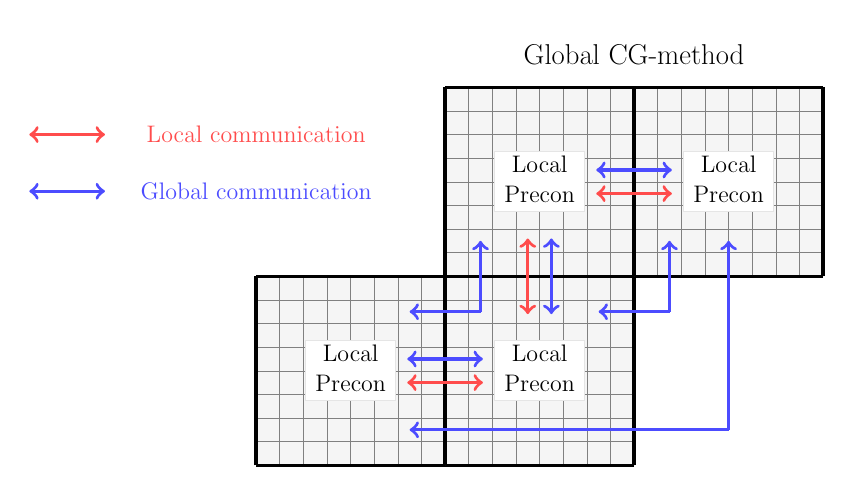
\begin{tikzpicture}
[
scale=0.6,
every node/.style={scale=0.6},
Background/.style={rectangle,draw=black!04,fill=black!04, thin, minimum size = 4 cm},
Obstruction/.style={rectangle,draw=black!70,fill=black!40, very thick, minimum size=1cm},
GlobalBorder/.style={-.,draw=black!100,  thin},
Finegrid/.style={step=0.5cm,gray,very thin},
Thickline/.style={-,draw=black!100,fill=black!02, very thick},
Thinline/.style={draw=black!100,fill=black!02, very thin},
Ball/.style={circle, draw=black!40, fill=red!20, thin, minimum size=3.5mm},
Circle/.style={circle,draw=black!40,fill=black!06,thin,minimum size=35.5mm},
Rectangle/.style={rectangle,draw=black!10,fill=white,inner xsep=0pt, inner ysep=0pt,},
Box/.style= {very thin, rectangle, inner xsep=10pt, inner ysep=10pt,},
DotBox/.style= {very thick, rectangle, inner xsep=0pt, inner ysep=8pt, dotted, fill=white, draw=black!70,},
ComRedArrow/.style= {very thick, draw=red!70,},
ComBlueArrow/.style= {very thick, draw=blue!70,},
DotArrow/.style= {<-, thick, dotted, draw=black!70,},
DotLine/.style= {very thick, dotted, draw=black!70,},
]

%\draw[GlobalBorder, fill=black!10] (-1.2,-1.2)--(13.2,-1.2)--(13.2,9.2)--(-1.2,9.2)--(-1.2,-1.2);
\node [Box, black] (box) at (8.0,8.7){\LARGE Global CG-method};

\node[Background] at (  2,2) {};
\node[Background] at (  6,2) {};
\node[Background] at (  6,6) {};
\node[Background] at (10,6) {};

\node[Obstruction] at (2,2) {};

\draw[Finegrid] (0,0) grid (  8,4);
\draw[Finegrid] (4,4) grid (12,8);

\draw[Thickline] (0,0)--(  8,0);
\draw[Thickline] (4,8)--(12,8);
\draw[Thickline] (0,4)--(  4,4);
\draw[Thickline] (8,4)--(12,4);

\draw[Thickline] (  0,0)--(  0,4);
\draw[Thickline] (  4,8)--(12,8);
\draw[Thickline] (  4,4)--(  4,8);
\draw[Thickline] (  8,0)--(  8,4);
\draw[Thickline] (12,4)--(12,8);

\draw[Thickline] (4,0)--(4,4);
\draw[Thickline] (4,4)--(8,4);
\draw[Thickline] (8,4)--(8,8);

\node[Rectangle] at (  2,2.0) {\Large \begin{tabular}{c} Local \\ Precon\end{tabular}};
\node[Rectangle] at (  6,2.0) {\Large \begin{tabular}{c} Local \\ Precon\end{tabular}};
\node[Rectangle] at (  6,6.0) {\Large \begin{tabular}{c} Local \\ Precon\end{tabular}};
\node[Rectangle] at (10,6.0) {\Large \begin{tabular}{c} Local \\ Precon\end{tabular}};

\draw[<->,ComRedArrow](3.2,1.75)--(4.8,1.75);
\draw[<->,ComRedArrow](5.75,3.2)--(5.75,4.8);
\draw[<->,ComRedArrow](7.2,5.75)--(8.8,5.75);

\draw[<->,ComBlueArrow](3.2,2.25)--(4.8,2.25);
\draw[<->,ComBlueArrow](6.25,3.2)--(6.25,4.8);
\draw[<->,ComBlueArrow](7.2,6.25)--(8.8,6.25);

\draw[<-, ComBlueArrow](3.25,3.25)--(4.75,3.25);
\draw[->, ComBlueArrow](4.75,3.25)--(4.75,4.75);
\draw[<-, ComBlueArrow](7.25,3.25)--(8.75,3.25);
\draw[->, ComBlueArrow](8.75,3.25)--(8.75,4.75);
\draw[<-, ComBlueArrow](3.25,0.75)--(10,0.75);
\draw[->, ComBlueArrow](10.0,0.75)--(10,4.75);

\draw[<->,ComRedArrow](-4.8,7.0)--(-3.2,7.0);
\node [Box,red!70] (box) at (-0.0,7.0){%
    \begin{minipage}{0.56\textwidth}
    \begin{center}
        {\Large Local communication}
    \end{center}
    \end{minipage}};
    
\draw[<->,ComBlueArrow](-4.8,5.8)--(-3.2,5.8);
\node [Box,blue!70] (box) at (-0.0,5.8){%
    \begin{minipage}{0.56\textwidth}
    \begin{center}
        {\Large Global communication}
    \end{center}
    \end{minipage}};
    

\end{tikzpicture}
